\documentclass[tikz]{standalone}
\usetikzlibrary{shapes.geometric}
\usepackage{tikz}
\usepackage{standalone}
\begin{document}
	
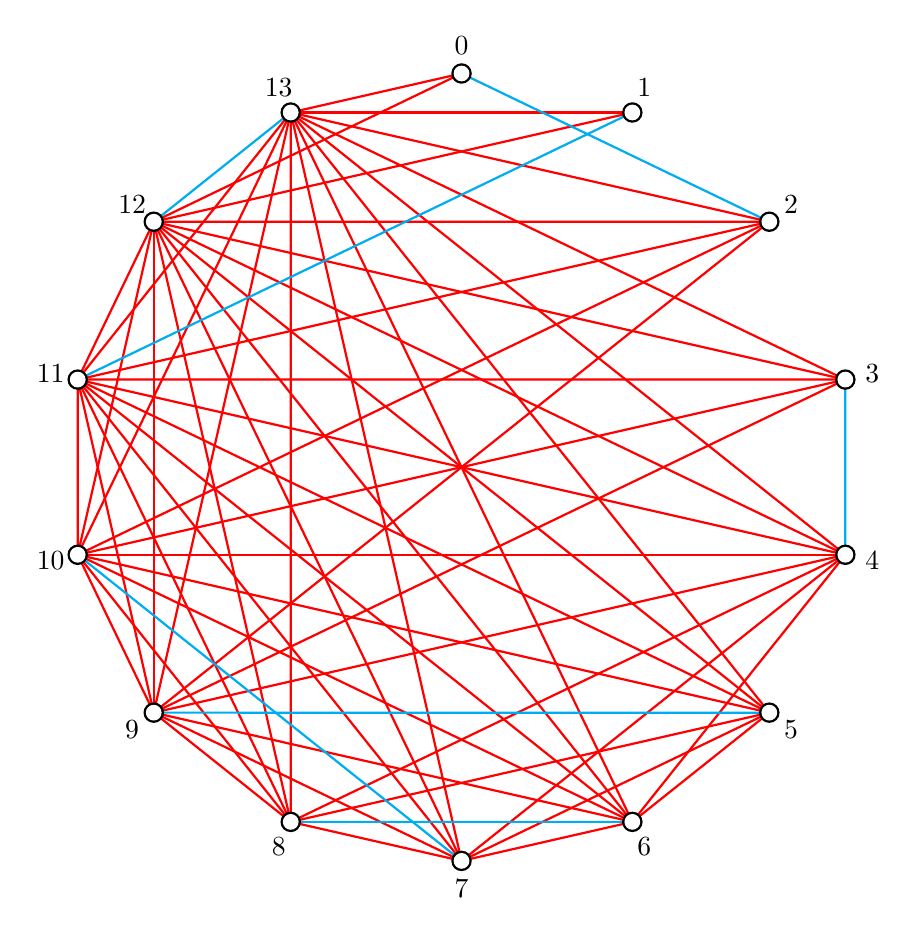
\begin{tikzpicture}
%Values of nodes:
% 0 = 1
% 1 = 1
% 2 = 2
% 3 = 2
% 4 = 3
% 5 = 3
% 6 = 4
% 7 = 4
% 8 = 4
% 9 = 5
% 10 = 5
% 11 = 6
% 12 = 7
% 13 = 7
% threshold tau = 7
%\draw [help lines] (-5,-2) grid (15, 13);

\foreach \n in {0,...,13}
	\fill (90-\n*25.71428571:5cm) coordinate (v\n) circle [radius = 0.1]
		++(90-\n*25.71428571:10pt) node {\n};
\foreach \m/\n in {0/13,0/12,1/13,1/12,2/13,2/12,2/11,2/10,2/9,3/13,3/12,3/11,3/10,3/9,4/13,4/12,4/11,4/10,4/9,4/8,4/7,4/6,5/13,5/12,5/11,5/10,5/8,5/7,5/6,6/13,6/12,6/11,6/10,6/9,6/7,7/13,7/12,7/11,7/9,7/8,8/13,8/12,8/11,8/10,8/9,9/13,9/12,9/11,9/10,10/13,10/12,10/11,11/13,11/12}	
	\draw [thick, red] (v\n) -- (v\m);
\foreach \m/\n in {0/2, 1/11, 3/4, 5/9, 6/8, 7/10, 12/13}
	\draw [thick, cyan] (v\n) -- (v\m);
\foreach \n in {0,...,13}
	\fill (90-\n*25.71428571:5cm) coordinate (v\n) circle [radius = 0.13];
\foreach \n in {0,...,13}
	\fill [white] (90-\n*25.71428571:5cm) coordinate (v\n) circle [radius = 0.1];

\end{tikzpicture}
	
\end{document}